%****************************************************************************************************************************************
% File: cps-ontology.tex
%
% This file is automatically generated. Please do not edit!
%****************************************************************************************************************************************
\section{Ontology Overview}

\todoAuthors{Provide ``rdfs:comment'' annotation in ontology}

Figure \ref{fig:cps_ontology_overview} shows an overview of the CPS ontology. The details of each concept are
provided in the following subsections.

\begin{figure}[!htb]
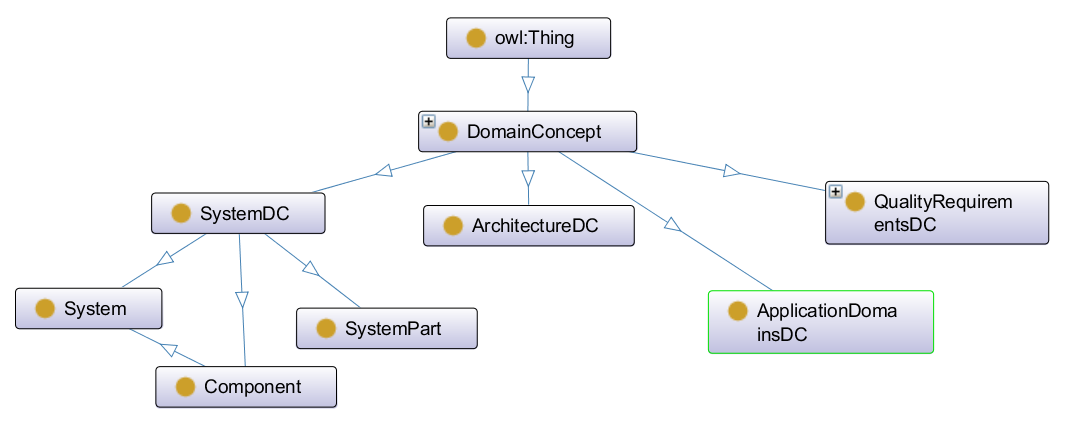
\includegraphics[width=\textwidth]{figures/cps_ontology_overview.png}
\caption{Overview of the CPS ontology}
\label{fig:cps_ontology_overview}
\end{figure}


	
\section{Domain Concepts}

This ontology of cyber-physical systems contains concepts divided into sub-domains as presented in the following subsections.

\subsection{ApplicationDomainsDC}
\label{subsecDC:ApplicationDomainsDC}

Various studies have addressed the domains and domain specific applications of CPS. Gunes et al. summarize a number of research efforts that address some of those domains, namely Smart Manufacturing, Emergency Response, Air Transportation, Critical Infrastructure, Health Care and Medicine, Intelligent Transportation, and Robotic for Service.

\subsubsection{ApplicationDomain}
\label{subsubsecC:ApplicationDomain}
\didx{ApplicationDomain}

\todoAuthors{Provide ``rdfs:comment'' annotation in ontology}

\textbf{Subclass of}
\begin{itemize}
	\item \textbf{ApplicationDomainsDC} (see section \ref{subsecDC:ApplicationDomainsDC})
\end{itemize}



\subsection{ArchitectureDC}
\label{subsecDC:ArchitectureDC}

\todoAuthors{Provide ``rdfs:comment'' annotation in ontology}





\subsection{QualityRequirementsDC}
\label{subsecDC:QualityRequirementsDC}

Cyber-Physical Systems revolutionize our interaction with the physical world. Of course, this revolution does not come free. Since even legacy embedded systems require higher standards than general-purpose computing, we need to pay special attention to this next generation physically-aware engineered system requirements if we really want to put our full trust in them. Therefore, we want to clarify the definitions of some common CPS system-level requirements /challenges.

\subsubsection{Accuracy}
\label{subsubsecC:Accuracy}
\didx{Accuracy}

Accuracy refers to the degree of closeness of a system's measured/observed outcome to its actual/calculated one. A highly accurate system should converge to the actual outcome as close as possible. High accuracy especially comes into play for CPS applications where even small imprecisions are likely to cause system failures. For example, a motion-based object tracking system under the presence of imperfect sensor conditions may take untimely control action based on incorrect object position estimation, which in return leads to the system failure.

\textbf{Subclass of}
\begin{itemize}
	\item \textbf{Predictability} (see section \ref{subsubsecC:Predictability})
\end{itemize}






\subsubsection{Adaptability}
\label{subsubsecC:Adaptability}
\didx{Adaptability}

Adaptability refers to the capability of a system to change its state to survive by adjusting its own configuration in response to different circumstances in the environment. A highly adaptable system should be quickly adaptable to evolving needs/circumstances. Adaptability is one of the key features in the next generation air transportation systems (e.g. NextGen). NextGen's capabilities enhance airspace performance with its computerized air transportation network which enables air vehicles immediately to accommodate themselves to evolving operational environment such as weather conditions, air vehicle routing and other pertinent flight trajectory patterns over satellites, air traffic congestion, and issues related to security.

\textbf{Subclass of}
\begin{itemize}
	\item \textbf{Sustainability} (see section \ref{subsubsecC:Sustainability})
\end{itemize}






\subsubsection{Availability}
\label{subsubsecC:Availability}
\didx{Availability}

Availability refers to the property of a system to be ready for access even when faults occur. A highly available system should isolate malfunctioning portion from itself and continue to operate without it. Malicious cyber-attacks (e.g. denial of service attacks) hinder availability of the system services significantly. For example, in Cyber-Physical Medical Systems, medical data shed light on necessary actions to be taken in a timely manner to save a patient's life. Malicious attacks or system/component failure may cause services providing such data to become unavailable, hence, posing risk on the patient's life.

\textbf{Subclass of}
\begin{itemize}
	\item \textbf{Dependability} (see section \ref{subsubsecC:Dependability})
	\item \textbf{Security} (see section \ref{subsubsecC:Security})
\end{itemize}






\subsubsection{Composibility}
\label{subsubsecC:Composibility}
\didx{Composibility}

Composibility refers to the property of several components to be merged within a system and their inter-relationships. A highly composable system should allow recombination of the system components repeatedly to satisfy specific system requirements. Composibility should be examined in different levels (e.g. device composibility, code composibility, service composibility, system composibility). Certainly, system composibility is more challenging, hence the need for well-defined composition methodologies that follow composition properties from the bottom up. Additionally, requirements and evaluations must be composable accordingly. In the future, it will probably be of paramount importance to incrementally add emerging systems to the system of systems (e.g. CPS) with some predictable confidence without degrading the operation of the resulting  system.

\textbf{Subclass of}
\begin{itemize}
	\item \textbf{Interoperability} (see section \ref{subsubsecC:Interoperability})
\end{itemize}






\subsubsection{Compositonality}
\label{subsubsecC:Compositonality}
\didx{Compositonality}

Compositionality refers to the property of how well a system can be understood entirely by examining every part of it. A highly compositional system should provide great insight about the whole from derived behaviors of its constituent parts/components. Achieving high compositionality in CPS design is very challenging especially due to the chaotic behavior of constituent physical subsystems. Designing highly compositional CPS involves strong reasoning about the behavior of all constituent cyber and physical subsystems/components and devising cyber-physical methodologies for assembling CPSs from individual cyber and physical components, while requiring precise property taxonomies, formal metrics and standard test benches for their evaluation, and well-defined mathematical models of the overall system and its constituents.

\textbf{Subclass of}
\begin{itemize}
	\item \textbf{Predictability} (see section \ref{subsubsecC:Predictability})
\end{itemize}






\subsubsection{Confidentiality}
\label{subsubsecC:Confidentiality}
\didx{Confidentiality}

Confidentiality refers to the property of allowing only the authorized parties to access sensitive information generated within the system. A highly confidential system should employ the most secure methods of protection from unauthorized access, disclosure, or tampering. Data confidentiality is an important issue that needs to be satisfied in most CPS applications. For example, in an emergency management sensor network, attacks targeting confidentiality of data transmitted may degrade effectiveness of an emergency management system. Confidentiality of data transmitted through attacked sensor nodes can be compromised and that can cause data flow in the network to be directed over compromised sensors; critical data to be eavesdropped; or fake node identities to be generated in the network. Further, false/malicious data can be injected into the network over those fake nodes. Therefore, confidentiality of data circulation needs to be retained in a reasonable degree.

\textbf{Subclass of}
\begin{itemize}
	\item \textbf{Security} (see section \ref{subsubsecC:Security})
\end{itemize}






\subsubsection{Dependability}
\label{subsubsecC:Dependability}
\didx{Dependability}

Dependability refers to the property of a system to perform required functionalities during its operation without significant degradation in its performance and outcome. Dependability reflects the degree of trust put in the whole system. A highly dependable system should operate properly without intrusion, deliver requested services as specified and not fail during its operation. The words dependability and trustworthiness are often used interchangeably. Assuring dependability before actual system operation is a very difficult task to achieve. For example, timing uncertainties regarding sensor readings and prompt actuation may degrade dependability and lead to unanticipated consequences. Cyber and physical components of the system are inherently interdependent and those underlying components might be dynamically interconnected during system operation, which, in return, renders dependability analysis very difficult. A common language to express dependability related information across constituent systems/underlying components should be introduced in the design stage.

\textbf{Subclass of}
\begin{itemize}
	\item \textbf{QualityRequirementsDC} (see section \ref{subsecDC:QualityRequirementsDC})
\end{itemize}






\subsubsection{Efficiency}
\label{subsubsecC:Efficiency}
\didx{Efficiency}

Efficiency refers to the amount of resources (such as energy, cost, time etc.) the system requires to deliver specified functionalities. A highly efficient system should operate properly under optimum amount of system resources. Efficiency is especially important for energy management in CPS applications. For example, smart buildings can detect the absence of occupants and turn off HVAC (Heating, Ventilation, and Air Conditioning) units to save energy. Further, they can provide automated pre-heating or pre-cooling services based on the occupancy prediction techniques.

\textbf{Subclass of}
\begin{itemize}
	\item \textbf{Sustainability} (see section \ref{subsubsecC:Sustainability})
\end{itemize}






\subsubsection{Heterogeneity}
\label{subsubsecC:Heterogeneity}
\didx{Heterogeneity}

Heterogeneity refers to the property of a system to incorporate a set of different types of interacting and interconnected components forming a complex whole. CPSs are inherently heterogeneous due to constituent physical dynamics, computational elements, control logic, and deployment of diverse communication technologies. Therefore, CPSs necessitate heterogeneous composition of all system components. For example, incorporating heterogeneous computing and communication capabilities, future medical devices are likely to be interconnected in increasingly complex open systems with a plug-and-play fashion, which makes a heterogeneous control network and closed loop control of interconnected devices crucial. Configuration of such devices may be highly dynamic depending on patient-specific medical considerations. Enabled by the science and emerging technologies, medical systems of the future are expected to provide situation-aware component autonomy, cooperative coordination, real-time guarantee, and heterogeneous personalized configurations far more capable and complex than today's.

\textbf{Subclass of}
\begin{itemize}
	\item \textbf{Interoperability} (see section \ref{subsubsecC:Interoperability})
\end{itemize}






\subsubsection{Integrity}
\label{subsubsecC:Integrity}
\didx{Integrity}

Integrity refers to the property of a system to protect itself or information within it from unauthorized manipulation or modification to preserve correctness of the information. A high integrity system should provide extensive authorization and consistency check mechanisms. High integrity is one of the important properties of a CPS. CPSs need to be developed with greater assurance by providing integrity check mechanisms on several occasions (such as data integrity of network packets, distinguishing malicious behaviors from the ambient noise, identifying false data injection and compromised sensor/actuator components etc.). Properties of the physical and cyber processes should be well-understood and thus can be utilized to define required integrity assurance.

\textbf{Subclass of}
\begin{itemize}
	\item \textbf{Security} (see section \ref{subsubsecC:Security})
\end{itemize}






\subsubsection{Interoperability}
\label{subsubsecC:Interoperability}
\didx{Interoperability}

Interoperability refers to the ability of the systems/components to work together, exchange information and use this information to provide specified services. A highly interoperable system should provide or accept services conducive to effective communication and interoperation among system components. Performing far-reaching battlefield operations and having more interconnected and potentially joint-service combat systems, Unmanned Air Vehicles (UAVs) call for seamless communication between each other and numerous ground vehicles in operation. The lack of interoperability standards often causes reduction in the effectiveness of complicated and critical missions. Likewise, according to changing needs, dynamic standards should be developed and tested for devices, systems, and processes used in the Smart Grid to ensure and certify the interoperability of those ones being considered for a specific Smart Grid deployment under realistic operating conditions.

\textbf{Subclass of}
\begin{itemize}
	\item \textbf{QualityRequirementsDC} (see section \ref{subsecDC:QualityRequirementsDC})
\end{itemize}






\subsubsection{Maintainability}
\label{subsubsecC:Maintainability}
\didx{Maintainability}

Maintainability refers to the property of a system to be repaired in case a failure occurs. A highly maintainable system should be repaired in a simple and rapid manner at the minimum expenses of supporting resources, and free from causing additional faults during the maintenance process. With the close interaction among the system components (e.g. sensors, actuators, cyber components, and physical components) underlying CPS infrastructure, autonomous predictive /corrective diagnostic mechanisms can be proposed. Continuous monitoring and testing of the infrastructure can be performed through those mechanisms. The outcome of monitoring and testing facilities help finding which units need to be repaired. Some components, which happen to be the source of recurrent failures, can be redesigned or discarded and replaced with the ones with better quality

\textbf{Subclass of}
\begin{itemize}
	\item \textbf{Dependability} (see section \ref{subsubsecC:Dependability})
\end{itemize}






\subsubsection{Predictability}
\label{subsubsecC:Predictability}
\didx{Predictability}

Predictability refers to the degree of foreseeing of a system's state/behavior/functionality either qualitatively or quantitatively. A highly predicable system should guarantee the specified outcome of the system's behavior/functionality to a great extent every moment of time at which it is operating while meeting all system requirements. In Cyber-Physical Medical Systems (CPMS), smart medical devices together with sophisticated control technologies are supposed to be well adapted to the patient's conditions, predict the patient's movements, and change their characteristics based on context awareness within the surrounding environment. Many medical devices perform operations in real-time, satisfying different timing constraints and showing diverse sensitivity to timing uncertainties (e.g. delays, jitters etc.). However, not all components of CPMS are time-predictable. Therefore, in addition to new programming and networking abstractions, new policies of resource allocation and scheduling should be developed to ensure predictable end-to-end timing constraints.

\textbf{Subclass of}
\begin{itemize}
	\item \textbf{QualityRequirementsDC} (see section \ref{subsecDC:QualityRequirementsDC})
\end{itemize}






\subsubsection{Reconfigurability}
\label{subsubsecC:Reconfigurability}
\didx{Reconfigurability}

Reconfigurability refers to the property of a system to change its configurations in case of
failure or upon inner or outer requests. A highly reconfigurable system should be self-configurable, meaning able to fine-tune itself dynamically and coordinate the operation of its components at finer granularities. CPSs can be regarded as autonomously reconfigurable engineered systems. Remote monitoring and control mechanisms might be necessity in some CPS application scenarios such as international border monitoring, wildfire emergency management, gas pipeline monitoring etc. Operational needs (e.g. security threat level updates, regular code updates, efficient energy management etc.) may change for such scenarios, which calls for significant reconfiguration of sensor/actuator nodes being deployed or the entire network to provide the best possible service and use of resources.

\textbf{Subclass of}
\begin{itemize}
	\item \textbf{Sustainability} (see section \ref{subsubsecC:Sustainability})
\end{itemize}






\subsubsection{Reliability}
\label{subsubsecC:Reliability}
\didx{Reliability}

Reliability refers to the degree of correctness which a system provides to perform its function.
The certification of system capabilities about how to do things correctly does not mean that they are done correctly. So a highly reliable system makes sure that it does the things right. Considering the fact that CPSs are expected to operate reliably in open, evolving, and uncertain environments, uncertainty in the knowledge, attribute (e.g. timing), or outcome of a process in the CPS infrastructure makes it necessary to quantify uncertainties during the CPS design stage. That uncertainty analysis will yield to effective CPS reliability characterization. Besides, accuracy of physical and cyber components, potential errors in design/control flow, cross-domain network connections in an ad-hoc manner limit the CPS reliability.

\textbf{Subclass of}
\begin{itemize}
	\item \textbf{QualityRequirementsDC} (see section \ref{subsecDC:QualityRequirementsDC})
\end{itemize}






\subsubsection{Resilience}
\label{subsubsecC:Resilience}
\didx{Resilience}

Resilience refers to the ability of a system to persevere in its operation and delivery of services
in an acceptable quality in case the system is exposed to any inner or outer difficulties (e.g. sudden defect, malfunctioning components, rising workload etc.) that do not exceed its endurance limit. A highly resilient system should be self-healing and comprise early detection and fast recovery mechanisms against failures to continue to meet the demands for services. High resilience comes into play in delivering mission-critical services (e.g. automated brake control in vehicular CPS, air and oxygen flow control over an automated medical ventilator etc.). Mission-critical CPS applications are often required to operate even in case of disruptions at any level of the system (e.g. hardware, software, network connections, or the underlying infrastructure). Therefore, designing highly resilient CPS requires thorough understanding of potential failures and disruptions, the resilience properties of the pertinent application, and system evolution due to the dynamically changing nature of the operational environment.

\textbf{Subclass of}
\begin{itemize}
	\item \textbf{Sustainability} (see section \ref{subsubsecC:Sustainability})
\end{itemize}






\subsubsection{Robustness}
\label{subsubsecC:Robustness}
\didx{Robustness}

Robustness refers to the ability of a system to keep its stable configuration and withstand any
failures. A highly robust system should continue to operate in the presence of any failures without fundamental changes to its original configuration and prevent those failures from hindering or stopping its operation. In addition to failures, the presence of disturbances possibly arising from sensor noises, actuator inaccuracies, faulty communication channels, potential hardware errors or software bugs may degrade overall robustness of CPS. Lack of modeling integrated system dynamics (e.g. actual ambient conditions in which CPSs operate), evolved operational environment, or unforeseen events are other particular non-negligible factors, which might be unavoidable in the run-time, hence the need for robust CPS design.

\textbf{Subclass of}
\begin{itemize}
	\item \textbf{Reliability} (see section \ref{subsubsecC:Reliability})
\end{itemize}






\subsubsection{Safety}
\label{subsubsecC:Safety}
\didx{Safety}

Safety refers to the property of a system to not cause any harm, hazard or risk inside or outside of it during its operation. A very safe system should comply with both general and application-specific safety regulations to a great extent and deploy safety assurance mechanisms in case something went wrong. For example, among the goals for Smart Manufacturing (SM), point-in-time tracking of sustainable production and real-time management of processes throughout the factory yield to improved safety. Safety of manufacturing plants can be highly optimized through automated process control using embedded control systems and data collection frameworks (including sensors) across the manufacturing enterprise. Smart networked sensors could detect operational failures/anomalies and help prevention of catastrophic incidents due to those failures/anomalies.

\textbf{Subclass of}
\begin{itemize}
	\item \textbf{Dependability} (see section \ref{subsubsecC:Dependability})
\end{itemize}






\subsubsection{Scalability}
\label{subsubsecC:Scalability}
\didx{Scalability}

Scalability refers to the ability of a system to keep functioning well even in case of change in its size/increased workload, and take full advantage of it. The increase in the system throughput should be proportional to the increase in the system resources. A highly scalable system should provide scatter and gather mechanisms for workload balancing and effective communication protocols to improve the performance. Depending on their scale, CPSs may comprise over thousands of embedded computers, sensors, and actuators that must work together effectively. Scalable embedded many-core architectures with a programmable interconnect network can be deployed to deliver increasing compute demand in CPS. Further, a high performance and highly scalable infrastructure is needed to allow the entities of CPS to join and leave the existing network dynamically. In the presence of frequent data dissemination among those entities, dynamic software updates (i.e. changing the computer program in run-time) can help update CPS applications dynamically and use CPS resources more productively.

\textbf{Subclass of}
\begin{itemize}
	\item \textbf{Interoperability} (see section \ref{subsubsecC:Interoperability})
\end{itemize}






\subsubsection{Security}
\label{subsubsecC:Security}
\didx{Security}

Security refers to the property of a system to control access to the system resources and protect
sensitive information from unauthorized disclosures. A highly secure system should provide protection mechanisms against unauthorized modification of information and unauthorized withholding of resources, and must be free from disclosure of sensitive information to a great extent. CPSs are vulnerable to failures and attacks on both the physical and cyber sides, due to their scalability, complexity, and dynamic nature. Malicious attacks (e.g. eavesdropping, man-in-the-middle, denial-of-service, injecting fake sensor measurements or actuation requests etc.) can be directed to the cyber infrastructure (e.g. data management layer, communication infrastructure, decision making mechanisms etc.) or the physical components with the intent of disrupting the system in operation or stealing sensitive information. Making use of a large-scale network (such as the Internet), adopting insecure communication protocols, heavy use of legacy systems or rapid adoption of commercial off-the-shelf (COTS) technologies are other factors which make CPSs easily exposed to the security threats.

\textbf{Subclass of}
\begin{itemize}
	\item \textbf{QualityRequirementsDC} (see section \ref{subsecDC:QualityRequirementsDC})
\end{itemize}






\subsubsection{Sustainability}
\label{subsubsecC:Sustainability}
\didx{Sustainability}

Sustainability means being capable of enduring without compromising requirements of the system, while renewing the system's resources and using them efficiently. A highly sustainable system is a long lasting system which has self-healing and dynamic tuning capabilities under evolving circumstances. Sustainability from energy perspective is an important part of energy provision and management policies. For example, the Smart Grid facilitates energy distribution, management, and customization from the perspective of customers or service providers by incorporating green sources of energy extracted from the physical environment. However, intermittent energy supply and unknown/ill-defined load characterization hinders the efforts to maintain long-term operation of the Smart Grid. To maintain sustainability, the Smart Grid requires planning and operation under uncertainties, use of real-time performance measurements, dynamic optimization techniques for energy usage, environment-aware duty cycling of computing units, and devising self-contained energy distribution facilities (such as autonomous micro grids).

\textbf{Subclass of}
\begin{itemize}
	\item \textbf{QualityRequirementsDC} (see section \ref{subsecDC:QualityRequirementsDC})
\end{itemize}



\subsection{SystemDC}
\label{subsecDC:SystemDC}

\todoAuthors{Provide ``rdfs:comment'' annotation in ontology}

\subsubsection{Component}
\label{subsubsecC:Component}
\didx{Component}

\todoAuthors{Provide ``rdfs:comment'' annotation in ontology}

\textbf{Subclass of}
\begin{itemize}
	\item \textbf{SystemDC} (see section \ref{subsecDC:SystemDC})
\end{itemize}






\subsubsection{System}
\label{subsubsecC:System}
\didx{System}

\todoAuthors{Provide ``rdfs:comment'' annotation in ontology}

\textbf{Subclass of}
\begin{itemize}
	\item \textbf{Component} (see section \ref{subsubsecC:Component})
	\item \textbf{SystemDC} (see section \ref{subsecDC:SystemDC})
\end{itemize}






\subsubsection{SystemPart}
\label{subsubsecC:SystemPart}
\didx{SystemPart}

\todoAuthors{Provide ``rdfs:comment'' annotation in ontology}

\textbf{Subclass of}
\begin{itemize}
	\item \textbf{SystemDC} (see section \ref{subsecDC:SystemDC})
\end{itemize}

\section{Properties}


